% !Mode:: "TeX:UTF-8"

\chapter{用例模型}

\section{确定用例}

\subsection{系统用例}

\begin{figure}[htbp]

    \centering
    
    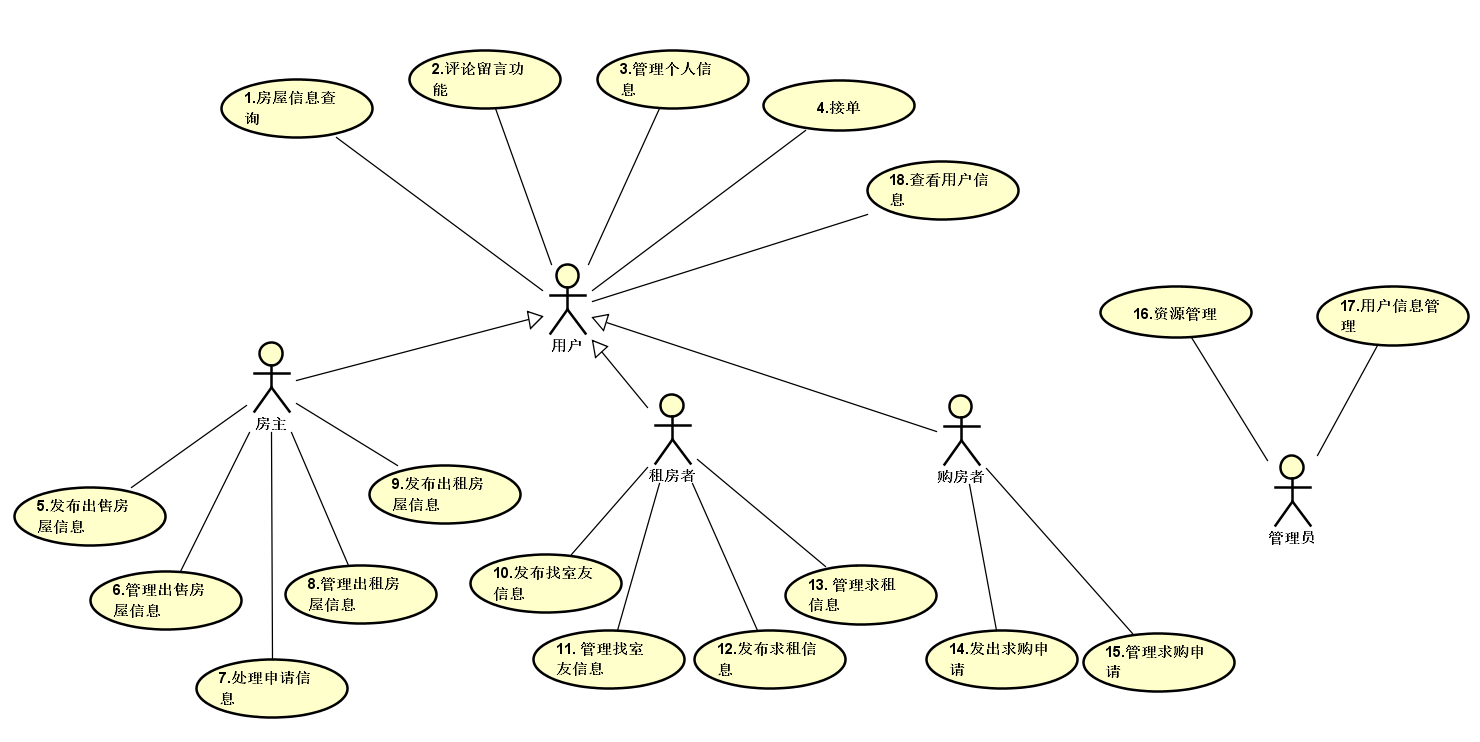
\includegraphics[height=10.0cm,width=14.0cm]{requirement/figures/xitong.png} 
    \caption{系统用例图}
    
    \end{figure}
\newpage
\subsection{用户}
 
\begin{figure}[htbp]

    \centering
    
    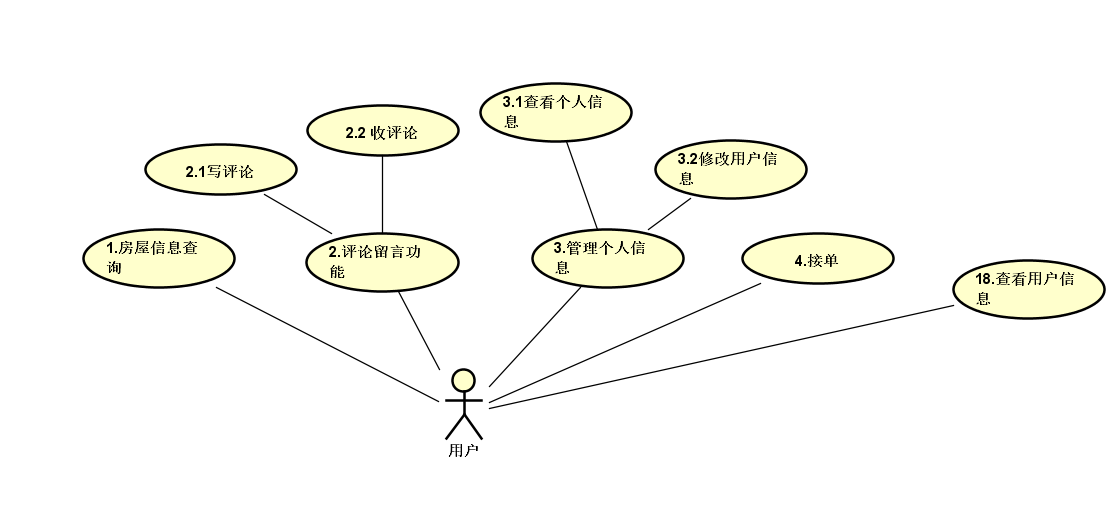
\includegraphics[height=10.0cm,width=14.0cm]{requirement/figures/yonghu.png} 
    \caption{用户用例图}
    
    \end{figure}
    \newpage
\subsection{房主}

\begin{figure}[htbp]

    \centering
    
    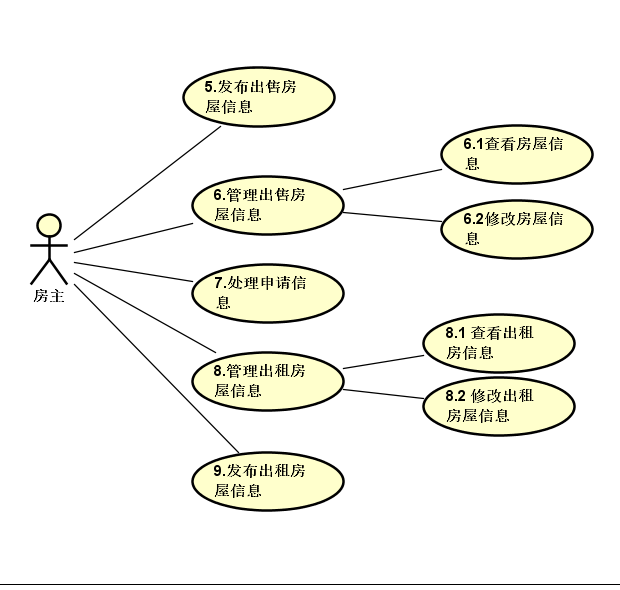
\includegraphics[height=14.0cm,width=14.0cm]{requirement/figures/fangzhu.png} 
    \caption{房主用例图}
    
    \end{figure}
    \newpage

\subsection{租房者}

\begin{figure}[htbp]

    \centering
    
    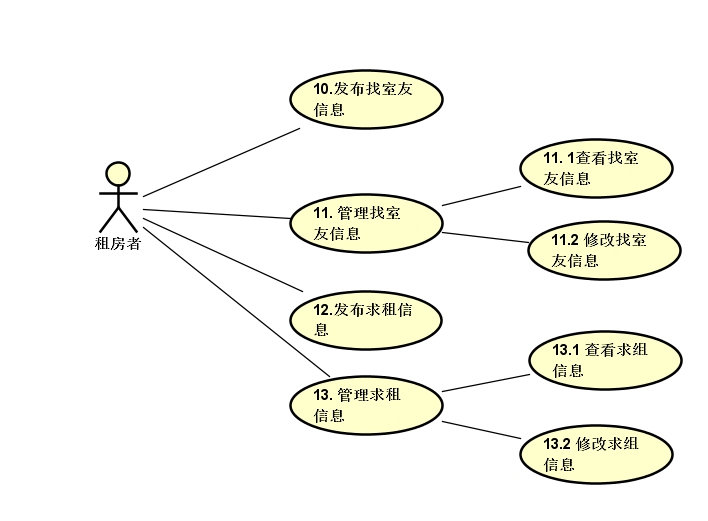
\includegraphics[height=14.0cm,width=14.0cm]{requirement/figures/zufangzhe.png} 
    \caption{租房者用例图}
    
    \end{figure}
    \newpage
\subsection{购房者}

\begin{figure}[htbp]

    \centering
    
    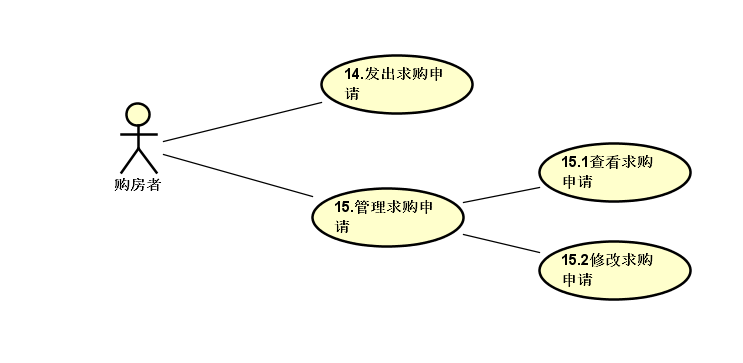
\includegraphics[height=12.0cm,width=14.0cm]{requirement/figures/goufangzhe.png} 
    \caption{购房者用例图}
    
    \end{figure}
    \newpage
\subsection{管理员}
 
\begin{figure}[htbp]

    \centering
    
    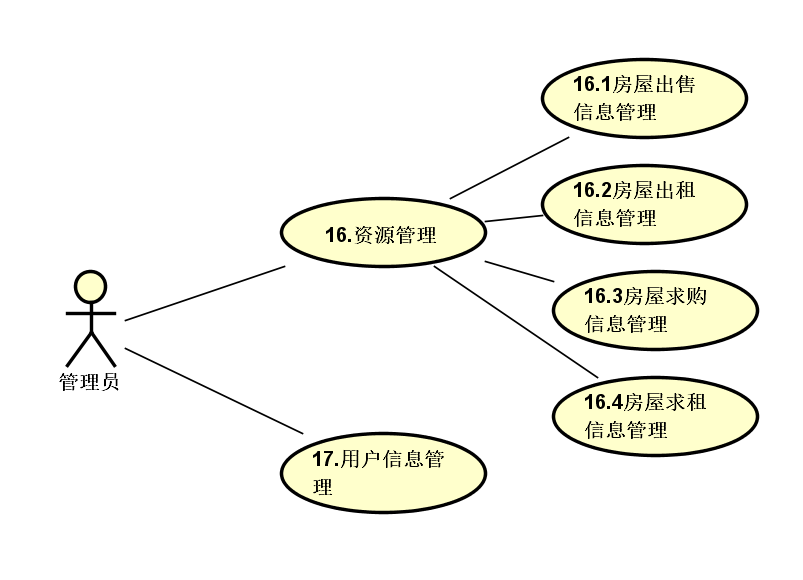
\includegraphics[height=14.0cm,width=14.0cm]{requirement/figures/guanliyuan.png} 
    \caption{管理员用例图}
    
    \end{figure}
    \newpage

\section{描述用例规约}

% \begin{table}[htbp]
% 	\centering
% 	\begin{tabular}{|c|l|c|l|}
%         \hline
%         编号 & 1 & 名称 & 房屋信息查询 \\ 
%         \hline
%         执行者 & \multicolumn{3}{|p{11cm}|}{用户} \\
%         \hline
%         描述 & \multicolumn{3}{|p{11cm}|}{
%             用户查询房屋信息,能够找到心仪的出租、出售、求租、求售、找室友帖子
%         } \\
%         \hline
%         前置条件 & \multicolumn{3}{|p{11cm}|}{无} \\
%         \hline
%         基本流程 & \multicolumn{3}{|p{11cm}|}{       
%             \begin{itemize}
%                 \item 1.选择房屋筛选条件
%                 \item 2.展示符合条件的房屋
%                 \item 3.点击可进入房屋详情页面进行申请
%             \end{itemize} \\
%         } \\
%         \hline
%         结束状况 & \multicolumn{3}{|p{11cm}|}{系统展示符合条件的房屋信息} \\
%         \hline
%         可选流程 & \multicolumn{3}{|p{11cm}|}{无} \\
%         \hline
%         异常流程 & \multicolumn{3}{|p{11cm}|}{无} \\
%         \hline
%         说明 & \multicolumn{3}{|p{11cm}|}{无} \\
%         \hline
%     \end{tabular}
%     \caption{房屋信息查询}
% \end{table}

\begin{table}[htbp]
	\centering
	\begin{tabular}{|c|p{11cm}|}
        \hline
        编号 & 1 \\
        \hline
        名称 & 房屋信息查询 \\ 
        \hline
        执行者 &用户 \\
        \hline
        描述 & 用户查询房屋信息,能够找到心仪的出租、出售、求租、求售、找室友帖子        \\
        \hline
        前置条件 & 无 \\
        \hline
        基本流程 & \begin{itemize}
            \item 1.选择房屋筛选条件
            \item 2.展示符合条件的房屋
            \item  3.点击可进入房屋详情页面进行申请
        \end{itemize} \\
        \hline
        结束状况 &系统展示符合条件的房屋信息 \\
        \hline
        可选流程 & 无 \\
        \hline
        异常流程 & 无 \\
        \hline
        说明 & 无 \\
        \hline
    \end{tabular}
    \caption{房屋信息查询}
\end{table}

\begin{table}[htbp]
	\centering
	\begin{tabular}{|c|p{11cm}|}
        \hline
        编号 & 2.1 \\
        \hline
        名称 & 写评论 \\ 
        \hline
        执行者 &用户 \\
        \hline
        描述 & 每个页面(包括出租出售求租求购找室友)下方具有评论区, 供用户在此交流.        \\
        \hline
        前置条件 & 用户打开相关页面 \\
        \hline
        基本流程 & \begin{itemize}
            \item 1.编辑文本框
            \item 2.点击发送
        \end{itemize} \\
        \hline
        结束状况 & 消息发送成功 \\
        \hline
        可选流程 & 用户可以选择新建评论, 或者回复其它用户的评论 \\
        \hline
        异常流程 & 无 \\
        \hline
        说明 & 无 \\
        \hline
    \end{tabular}
    \caption{写评论}
\end{table}

\begin{table}[htbp]
	\centering
	\begin{tabular}{|c|p{11cm}|}
        \hline
        编号 & 2.2 \\ 
        \hline
        名称 & 收评论 \\ 
        \hline
        执行者 &用户 \\
        \hline
        描述 & 当其它用户发出与此用户相关的评论时, 在微信的消息列表中发送提示.        \\
        \hline
        前置条件 & 无 \\
        \hline
        基本流程 & \begin{itemize}
            \item 1. 微信消息列表中查看提示
            \item 2. 点击消息后跳转至相关页面
        \end{itemize} \\
        \hline
        结束状况 & 跳转至相关页面. \\
        \hline
        可选流程 & 无 \\
        \hline
        异常流程 & 无 \\
        \hline
        说明 & 无 \\
        \hline
    \end{tabular}
    \caption{收评论}
\end{table}

\begin{table}[htbp]
	\centering
	\begin{tabular}{|c|p{11cm}|}
        \hline
        编号 & 3.1 \\
        \hline
        名称 & 查看个人信息 \\ 
        \hline
        执行者 &用户 \\
        \hline
        描述 & 在个人主页中用户可以查看个人信息       \\
        \hline
        前置条件 & 无 \\
        \hline
        基本流程 & \begin{itemize}
            \item 1.点击个人信息按钮
            \item 2.展示个人信息
        \end{itemize} \\
        \hline
        结束状况 & 展示个人信息页面 \\
        \hline
        可选流程 & 无 \\
        \hline
        异常流程 & 无 \\
        \hline
        说明 & 无 \\
        \hline
    \end{tabular}
    \caption{查看个人信息}
\end{table}

\begin{table}[htbp]
	\centering
	\begin{tabular}{|c|p{11cm}|}
        \hline
        编号 & 3.2 \\
        \hline
        名称 & 房屋信息查询修改个人信息 \\ 
        \hline
        执行者 &用户 \\
        \hline
        描述 & 可以在个人主页中编辑自身相关信息        \\
        \hline
        前置条件 & 用户已经登陆 \\
        \hline
        基本流程 & \begin{itemize}
            \item 1. 点击按钮
            \item 2. 编辑相关文本框
            \item  3. 提交
        \end{itemize} \\
        \hline
        结束状况 & 点击提交, 提示成功 \\
        \hline
        可选流程 & 无 \\
        \hline
        异常流程 & 无 \\
        \hline
        说明 & 无 \\
        \hline
    \end{tabular}
    \caption{修改个人信息}
\end{table}

\begin{table}[htbp]
	\centering
	\begin{tabular}{|c|p{11cm}|}
        \hline
        编号 & 4 \\
        \hline
        名称 & 接单 \\ 
        \hline
        执行者 &用户 \\
        \hline
        描述 & 用户可以对于其他用户发布的出租/出售/求购/求租/找室友的帖子进行接单 \\
        \hline
        前置条件 & 已有出租/出售/求购/求租/找室友的帖子 \\
        \hline
        基本流程 & \begin{itemize}
            \item 1.点击提示框
            \item 2.进入相应事务页面
            \item 3.发出接单申请
        \end{itemize} \\
        \hline
        结束状况 & 接单成功 \\
        \hline
        可选流程 & \begin{itemize}
            \item 1.出租帖子建立拼单队列
            \item 2.拼单成功
            \item 3.发出接单申请
        \end{itemize} \\
        \hline
        异常流程 & 无 \\
        \hline
        说明 & 无 \\
        \hline
    \end{tabular}
    \caption{接单}
\end{table}

\begin{table}[htbp]
	\centering
	\begin{tabular}{|c|p{11cm}|}
        \hline
        编号 & 5 \\
        \hline
        名称 & 发布出售房屋信息 \\ 
        \hline
        执行者 & 房主 \\
        \hline
        描述 & 房主用户可以发布出售房屋的相关信息,  以提供给买房者参考.        \\
        \hline
        前置条件 & 无 \\
        \hline
        基本流程 & \begin{itemize}
            \item 1.进入相关页面
            \item 2.编辑房屋信息, 卖房信息, 定价和介绍等相关信息
            \item 3.点击发布
        \end{itemize} \\
        \hline
        结束状况 & 发布成功 \\
        \hline
        可选流程 & 无 \\
        \hline
        异常流程 & 无 \\
        \hline
        说明 & 无 \\
        \hline
    \end{tabular}
    \caption{发布出售房屋信息}
\end{table}

\begin{table}[htbp]
	\centering
	\begin{tabular}{|c|p{11cm}|}
        \hline
        编号 & 1 \\
        \hline
        名称 & 查看出售房屋信息 \\ 
        \hline
        执行者 & 房主 \\
        \hline
        描述 & 查看自己所发布的出售房屋的相关信息        \\
        \hline
        前置条件 & 无 \\
        \hline
        基本流程 & \begin{itemize}
            \item 1.进入相关页面
            \item 2.查看
            
        \end{itemize} \\
        \hline
        结束状况 & 信息加载成功 \\
        \hline
        可选流程 & 无 \\
        \hline
        异常流程 & 无 \\
        \hline
        说明 & 无 \\
        \hline
    \end{tabular}
    \caption{查看出售房屋信息}
\end{table}

\begin{table}[htbp]
	\centering
	\begin{tabular}{|c|p{11cm}|}
        \hline
        编号 & 6.2 \\
        \hline
        名称 & 管理出售房屋信息 \\ 
        \hline
        执行者 & 房主 \\
        \hline
        描述 & 房主可以修改自己发布过的出售房屋的信息 \\
        \hline
        前置条件 & 已经发布过出售房屋信息 \\
        \hline
        基本流程 & \begin{itemize}
            \item 1.进入相关页面
            \item 2.点击相关文本框进行编辑
            \item  3.提交
        \end{itemize} \\
        \hline
        结束状况 & 提交成功 \\
        \hline
        可选流程 & 无 \\
        \hline
        异常流程 & 无 \\
        \hline
        说明 & 无 \\
        \hline
    \end{tabular}
    \caption{管理出售房屋信息}
\end{table}

\begin{table}[htbp]
	\centering
	\begin{tabular}{|c|p{11cm}|}
        \hline
        编号 & 7 \\
        \hline
        名称 & 处理申请信息 \\ 
        \hline
        执行者 & 房主 \\
        \hline
        描述 & 房主对求房者发出的求购求租申请进行回复处理\\
        \hline
        前置条件 & 求房者发出求购求租申请 \\
        \hline
        基本流程 & \begin{itemize}
            \item 1.查看求房者的求购求租申请
            \item 2.同意申请
            \item 3.订单完成
        \end{itemize} \\
        \hline
        结束状况 & 订单完成或取消 \\
        \hline
        可选流程 &  \begin{itemize}
            \item 拒绝申请
            \item 订单取消
        \end{itemize} \\
        \hline
        异常流程 & \begin{itemize}
            \item 求房者取消求购求租申请
            \item 订单取消
        \end{itemize} \\
        \hline
        说明 & 无 \\
        \hline
    \end{tabular}
    \caption{处理申请信息}
\end{table}

\begin{table}[htbp]
	\centering
	\begin{tabular}{|c|p{11cm}|}
        \hline
        编号 & 8.1 \\
        \hline
        名称 & 查看出租房屋信息 \\ 
        \hline
        执行者  房主 \\
        \hline
        描述 & 查看自己所发布的出租房屋的相关信息\\
        \hline
        前置条件 & 已经发布过出租房屋信息 \\
        \hline
        基本流程 & \begin{itemize}
            \item 1. 进入相关页面
            \item 2. 查看
 
        \end{itemize} \\
        \hline
        结束状况 & 信息加载成功 \\
        \hline
        可选流程 & 无 \\
        \hline
        异常流程 & 无 \\
        \hline
        说明 & 无 \\
        \hline
    \end{tabular}
    \caption{查看出租房屋信息}
\end{table}

\begin{table}[htbp]
	\centering
	\begin{tabular}{|c|p{11cm}|}
        \hline
        编号 & 8.2 \\
        \hline
        名称 & 修改出租房屋信息 \\ 
        \hline
        执行者 & 房主 \\
        \hline
        描述 & 房主可以修改自己发布过的出租房屋的信息 \\
        \hline
        前置条件 & 已经发布过出租房屋信息 \\
        \hline
        基本流程 & \begin{itemize}
            \item 1. 进入相关页面
            \item 2. 点击相关文本框进行编辑
            \item 3. 提交
        \end{itemize} \\
        \hline
        结束状况 & 提交成功 \\
        \hline
        可选流程 & 无 \\
        \hline
        异常流程 & 无 \\
        \hline
        说明 & 无 \\
        \hline
    \end{tabular}
    \caption{房屋信息查询}
\end{table}

\begin{table}[htbp]
	\centering
	\begin{tabular}{|c|p{11cm}|}
        \hline
        编号 & 9 \\
        \hline
        名称 & 发布出租房信息 \\ 
        \hline
        执行者 & 房主 \\
        \hline
        描述 & 可以发布出租房屋的相关信息, 以供租房者参考\\
        \hline
        前置条件 & 无 \\
        \hline
        基本流程 & \begin{itemize}
            \item 1. 进入相关页面
            \item 2. 编辑房屋信息, 定价, 介绍等相关信息
            \item 3. 提交
        \end{itemize} \\
        \hline
        结束状况 & 提交成功 \\
        \hline
        可选流程 & 无 \\
        \hline
        异常流程 & 无 \\
        \hline
        说明 & 无 \\
        \hline
    \end{tabular}
    \caption{发布出租房信息}
\end{table}

\begin{table}[htbp]
	\centering
	\begin{tabular}{|c|p{11cm}|}
        \hline
        编号 & 10 \\
        \hline
        名称 & 发布找室友信息 \\ 
        \hline
        执行者 & 租房者 \\
        \hline
        描述 & 已租到房或尚未租房的租房者寻找室友分担房屋租金 \\
        \hline
        前置条件 & 无 \\
        \hline
        基本流程 & \begin{itemize}
            \item 1.编辑寻找室友标准,已租房屋信息(已租到房)或目标租屋标准(尚未租房)等相关信息
            \item 2.点击发布
        \end{itemize} \\
        \hline
        结束状况 & 发布成功 \\
        \hline
        可选流程 & 无 \\
        \hline
        异常流程 & 无 \\
        \hline
        说明 & 无 \\
        \hline
    \end{tabular}
    \caption{发布找室友信息}
\end{table}

\begin{table}[htbp]
	\centering
	\begin{tabular}{|c|p{11cm}|}
        \hline
        编号 & 11.1 \\
        \hline
        名称 & 查看找室友信息 \\ 
        \hline
        执行者 & 租房者 \\
        \hline
        描述 & 查看自己发布的找室友的信息 \\
        \hline
        前置条件 & 本用户发布过找室友信息 \\
        \hline
        基本流程 & \begin{itemize}
            \item 1.点击我的事务
            \item 2.点击相应找室友事务
 
        \end{itemize} \\
        \hline
        结束状况 &跳转到找室友信息的界面 \\
        \hline
        可选流程 & 无 \\
        \hline
        异常流程 & 无 \\
        \hline
        说明 & 无 \\
        \hline
    \end{tabular}
    \caption{查看找室友信息}
\end{table}

\begin{table}[htbp]
	\centering
	\begin{tabular}{|c|p{11cm}|}
        \hline
        编号 & 11.2 \\
        \hline
        名称 & 修改找室友信息 \\ 
        \hline
        执行者 & 租房者 \\
        \hline
        描述 & 修改自己发布的找室友的信息\\
        \hline
        前置条件 & 本用户发布过找室友信息 \\
        \hline
        基本流程 & \begin{itemize}
            \item 1.点击我的事务
            \item 2.点击相应找室友事务
            \item 3.修改选定内容
        \end{itemize} \\
        \hline
        结束状况 &找室友信息发生改变 \\
        \hline
        可选流程 & 无 \\
        \hline
        异常流程 & 无 \\
        \hline
        说明 & 无 \\
        \hline
    \end{tabular}
    \caption{修改找室友信息}
\end{table}

\begin{table}[htbp]
	\centering
	\begin{tabular}{|c|p{11cm}|}
        \hline
        编号 & 12 \\
        \hline
        名称 & 发布求租信息 \\ 
        \hline
        执行者 & 租房者 \\
        \hline
        描述 & 已租到房或尚未租房的租房者寻找室友分担房屋租金 \\
        \hline
        前置条件 & 无 \\
        \hline
        基本流程 & \begin{itemize}
            \item 1. 进入相关页面
            \item 2. 点击相关文本框进行编辑
            \item 3. 提交
        \end{itemize} \\
        \hline
        结束状况 &发布成功 \\
        \hline
        可选流程 & 无 \\
        \hline
        异常流程 & 无 \\
        \hline
        说明 & 无 \\
        \hline
    \end{tabular}
    \caption{发布求租信息}
\end{table}

\begin{table}[htbp]
	\centering
	\begin{tabular}{|c|p{11cm}|}
        \hline
        编号 & 13.1 \\
        \hline
        名称 & 查看求租信息 \\ 
        \hline
        执行者 &租房者 \\
        \hline
        描述 & 查看自己发布的求租信息 \\
        \hline
        前置条件 & 本用户发布过求租信息 \\
        \hline
        基本流程 & \begin{itemize}
            \item 1.点击我的事务
            \item 2.点击相应求租事务
 
        \end{itemize} \\
        \hline
        结束状况 & 页面跳转到指定求租事务 \\
        \hline
        可选流程 & 无 \\
        \hline
        异常流程 & 无 \\
        \hline
        说明 & 无 \\
        \hline
    \end{tabular}
    \caption{查看求租信息}
\end{table}

\begin{table}[htbp]
	\centering
	\begin{tabular}{|c|p{11cm}|}
        \hline
        编号 & 13.2 \\
        \hline
        名称 & 修改求租信息 \\ 
        \hline
        执行者 & 租房者 \\
        \hline
        描述 & 租房者修改自己发布的求租信息 \\
        \hline
        前置条件 & 本用户发布过求租信息 \\
        \hline
        基本流程 & \begin{itemize}
            \item 1.点击我的事务
            \item 2.点击相应求租事务
            \item 3.修改选定内容
        \end{itemize} \\
        \hline
        结束状况 & 被选定的求租事务内容发生改变 \\
        \hline
        可选流程 & 无 \\
        \hline
        异常流程 & 无 \\
        \hline
        说明 & 无 \\
        \hline
    \end{tabular}
    \caption{修改求租信息}
\end{table}

\begin{table}[htbp]
	\centering
	\begin{tabular}{|c|p{11cm}|}
        \hline
        编号 & 14 \\
        \hline
        名称 & 发布求购申请 \\ 
        \hline
        执行者 & 租房者 \\
        \hline
        描述 & 租房者可以发布购房请求, 以供房主参考\\
        \hline
        前置条件 & 无 \\
        \hline
        基本流程 & \begin{itemize}
            \item 1. 进入相关页面
            \item 2. 编辑预期房屋信息, 预期定价等相关信息
            \item 3. 提交
        \end{itemize} \\
        \hline
        结束状况 & 提交成功 \\
        \hline
        可选流程 & 无 \\
        \hline
        异常流程 & 无 \\
        \hline
        说明 & 无 \\
        \hline
    \end{tabular}
    \caption{发布求购申请}
\end{table}

\begin{table}[htbp]
	\centering
	\begin{tabular}{|c|p{11cm}|}
        \hline
        编号 & 15.1 \\
        \hline
        名称 & 查看求购申请 \\ 
        \hline
        执行者 & 购房者 \\
        \hline
        描述 & 购房者查看自己所发布的求购房屋的相关信息 \\
        \hline
        前置条件 & 已经发布过求购申请 \\
        \hline
        基本流程 & \begin{itemize}
            \item 1. 进入相关页面
            \item 2. 查看
        \end{itemize} \\
        \hline
        结束状况 & 页面加载出相关数据 \\
        \hline
        可选流程 & 无 \\
        \hline
        异常流程 & 无 \\
        \hline
        说明 & 无 \\
        \hline
    \end{tabular}
    \caption{查看求购申请}
\end{table}

\begin{table}[htbp]
	\centering
	\begin{tabular}{|c|p{11cm}|}
        \hline
        编号 & 15.2 \\
        \hline
        名称 & 修改求购申请 \\ 
        \hline
        执行者 & 购房者 \\
        \hline
        描述 & 购房者对自己的求购信息进行 \\
        \hline
        前置条件 & 无 \\
        \hline
        基本流程 & \begin{itemize}
            \item 1. 进入相关页面
            \item 2. 点击相关文本框进行修改编辑
            \item 3. 提交
        \end{itemize} \\
        \hline
        结束状况 & 提交成功 \\
        \hline
        可选流程 & 无 \\
        \hline
        异常流程 & 无 \\
        \hline
        说明 & 无 \\
        \hline
    \end{tabular}
    \caption{修改求购申请}
\end{table}

\begin{table}[htbp]
	\centering
	\begin{tabular}{|c|p{11cm}|}
        \hline
        编号 & 16.1 \\
        \hline
        名称 & 房屋出售信息管理 \\ 
        \hline
        执行者 & 管理员 \\
        \hline
        描述 & 管理员对房主发布的出售信息进行管理,对无关信息、明显异常的信息进行删除\\
        \hline
        前置条件 & 无 \\
        \hline
        基本流程 & \begin{itemize}
            \item 1. 打开房屋出售信息管理界面
            \item 2. 对房屋信息进行筛查,审核
            \item 3.点击提交
        \end{itemize} \\
        \hline
        结束状况 & 提交成功 \\
        \hline
        可选流程 & 无 \\
        \hline
        异常流程 & 无 \\
        \hline
        说明 & 无 \\
        \hline
    \end{tabular}
    \caption{房屋出售信息管理}
\end{table}

\begin{table}[htbp]
	\centering
	\begin{tabular}{|c|p{11cm}|}
        \hline
        编号 & 16.2 \\
        \hline
        名称 & 房屋出租信息管理 \\ 
        \hline
        执行者 & 管理员 \\
        \hline
        描述 & 管理员对房主发布的出租信息进行管理,对无关信息、明显异常的信息进行删除     \\
        \hline
        前置条件 & 无 \\
        \hline
        基本流程 & \begin{itemize}
            \item 1.打开房屋出租信息管理界面
            \item 2.对房屋信息进行筛查,审核
            \item 3.点击提交
        \end{itemize} \\
        \hline
        结束状况 & 提交成功 \\
        \hline
        可选流程 & 无 \\
        \hline
        异常流程 & 无 \\
        \hline
        说明 & 无 \\
        \hline
    \end{tabular}
    \caption{房屋信息查询}
\end{table}

\begin{table}[htbp]
	\centering
	\begin{tabular}{|c|p{11cm}|}
        \hline
        编号 & 16.3 \\
        \hline
        名称 & 房屋求购信息管理 \\ 
        \hline
        执行者 & 管理员 \\
        \hline
        描述 & 管理员对求购者发布的求购信息进行管理,对无关信息、明显异常的信息进行删除 \\
        \hline
        前置条件 & 无 \\
        \hline
        基本流程 & \begin{itemize}
            \item 1. 打开房屋求购信息管理界面
            \item  2. 对求购信息进行筛查,审核
            \item  3.点击提交
        \end{itemize} \\
        \hline
        结束状况 & 提交成功 \\
        \hline
        可选流程 & 无 \\
        \hline
        异常流程 & 无 \\
        \hline
        说明 & 无 \\
        \hline
    \end{tabular}
    \caption{房屋求购信息管理}
\end{table}

\begin{table}[htbp]
	\centering
	\begin{tabular}{|c|p{11cm}|}
        \hline
        编号 & 16.4 \\
        \hline
        名称 & 房屋求购信息管理 \\ 
        \hline
        执行者 & 管理员 \\
        \hline
        描述 & 管理员对求租者发布的求租信息进行管理,对无关信息、明显异常的信息进行删除\\
        \hline
        前置条件 & 无 \\
        \hline
        基本流程 & \begin{itemize}
            \item 1. 打开房屋求购信息管理界面
            \item 2. 对求购信息进行筛查,审核
            \item 3.点击提交, 
        \end{itemize} \\
        \hline
        结束状况 & 提示成功 \\
        \hline
        可选流程 & 无 \\
        \hline
        异常流程 & 无 \\
        \hline
        说明 & 无 \\
        \hline
    \end{tabular}
    \caption{房屋求购信息管理}
\end{table}

\begin{table}[htbp]
	\centering
	\begin{tabular}{|c|p{11cm}|}
        \hline
        编号 & 17 \\
        \hline
        名称 & 用户信息管理 \\ 
        \hline
        执行者 &管理员 \\
        \hline
        描述 & 管理员对用户基本信息进行管理,对无关信息、明显异常的信息进行删除 \\
        \hline
        前置条件 & 无 \\
        \hline
        基本流程 & \begin{itemize}
            \item 1. 打开用户管理界面

            \item 2. 对用户信息进行核实,审批.
            
            \item 3. 点击提交
        \end{itemize} \\
        \hline
        结束状况 & 提示成功 \\
        \hline
        可选流程 & 无 \\
        \hline
        异常流程 & 无 \\
        \hline
        说明 & 无 \\
        \hline
    \end{tabular}
    \caption{房屋信息查询}
\end{table}

